% Target file: chapters/03_methodology_requirements.tex
%
% This chapter requires the following verified bibliography keys:
% iso29148, iso25010, eu2016gdpr, eu2001infosoc, pineau2021
%
% It also expects the following rendered figure:
% figures/rendered/research_cycle.pdf

\chapter{Research Methodology and Requirements}
\label{chap:methodology}

\begin{chapterplan}
  {8--10 pages}
  {Justify the research approach, describe the iterative process, derive testable requirements, and connect the research questions to artefact components and experiments.}
Primary evidence: design-science literature, the archived repository, supervisor traceability records, project design documents, formative evaluations, and reproducibility records.
\end{chapterplan}

\section{Introduction}
\label{sec:methodology-introduction}

The focus here is the way the project was investigated. Implementation details are deferred to \cref{chap:implementation}; this chapter instead explains the research approach, reconstructs the development sequence, and converts broad project aims into requirements that can be checked. I follow the principle in ISO/IEC/IEEE 29148 that a requirement should state observable behaviour together with a means of verification \parencite{iso29148}.

Although the two modes share the same application shell, they answer different technical questions. Document mode ingests anatomy PDFs and may return an answer, source records, and figures. The 3D mode resolves a structure against a geometry-oriented catalogue and uses an MCP toolchain to invoke Blender, producing a GLB, annotations, and a viewer URL. I keep their sources, failure modes, and evidence separate throughout the method because combining them would make later results difficult to interpret.

The requirements changed as the prototype changed. Research questions and supervisor feedback supplied the initial direction, while repository inspection and formative use exposed requirements that had not been visible at the outset.
\footnote{Project evidence: \codepath{project_resources/ARCHITECTURE_FOR_DIAGRAMS.md}, \codepath{project_resources/THESIS_SYSTEM_DESIGN_AND_MCP.md}, \codepath{project_resources/PROFESSOR_REQUIREMENTS_TRACEABILITY.md}, and \codepath{project_resources/EVALUATION_DATA_SUMMARY.md}.}

\section{Research Approach and Justification}
\label{sec:research-approach}

\subsection{Design-Science Orientation}
\label{subsec:design-science-orientation}

The research problem is constructive: the study asks how an anatomy assistant can be built so that document answers remain traceable and 3D actions leave inspectable evidence. A design-science orientation fits this problem because building and evaluating the artefact generates knowledge about both the proposed intervention and the setting in which it is used \parencite{hevner2004}.

The six activities described by \textcite{peffers2007} can be recognised in the project, but they did not occur as one orderly sequence. Demonstrations repeatedly sent the work back to design: exact terminology was missed, references were duplicated, local asset paths failed away from the development machine, and the first Blender outputs had weak anatomy provenance. Each problem changed either the artefact or the standard used to judge it. This iterative pattern is close to Wieringa's distinction between designing a treatment and investigating its behaviour in context \parencite{wieringa2014}.

\begin{figure}[htbp]
  \centering
  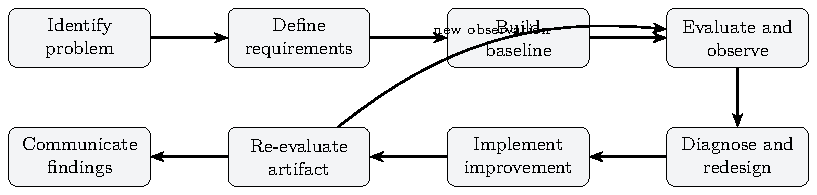
\includegraphics[
    width=0.74\textwidth,
    height=0.32\textheight,
    keepaspectratio
  ]{figures/rendered/research_cycle.pdf}
  \caption{Iterative design-science process used in the project. Formative observations generated revised requirements before final evaluation.}
  \label{fig:research-cycle}
\end{figure}

\subsection{Artefact, Evaluation Object, and Boundaries}
\label{subsec:artifact-evaluation-boundaries}

The artefact extends beyond the chat interface. It includes PDF ingestion, text and image indexes, retrieval and generation services, storage handling, the MCP host and client, the anatomy tool server, the export catalogue, Blender scripts, generated files, and the browser viewer.
\footnote{Project evidence: \codepath{project_resources/THESIS_SYSTEM_DESIGN_AND_MCP.md}; implementation locations are mapped in \cref{chap:implementation}.}
The evaluation object is their behaviour during defined tasks: ordinary anatomy questions, unsupported requests, ambiguous structure names, and selected technical failures.

The intended contribution has three parts: the dual-pipeline artefact, the measurements and failure cases retained from evaluation, and the engineering knowledge gained from designs that were kept, revised, or abandoned. These claims require different evidence. A class or endpoint can show that something was implemented; improvement requires a comparison and a recorded outcome \parencite{hevner2004,wieringa2014}.

The study remains a prototype investigation. It can examine retrieval, source linkage, figure delivery, catalogue resolution, artefact generation, and error handling. It was not designed to establish clinical validity or learning outcomes. In an educational anatomy setting, that limitation matters because fluent errors and over-reliance can affect learners who are not yet able to challenge the system \parencite{ji2023,kasneci2023}.

\section{Actual Iterative Research Process}
\label{sec:research-process}

The first working baseline used dense document retrieval. PDF text was chunked, embedded, stored in Chroma, and passed to a language model after similarity search. That simple route was useful because its weaknesses appeared quickly: exact terms were missed, repeated chunks crowded the source list, weak passages supported confident answers, and image-heavy material was poorly represented.
\footnote{Project evidence: \codepath{project_resources/THESIS_RESEARCH_LOG.docx} and \codepath{project_resources/EVALUATION_DATA_SUMMARY.md}.}

The next changes were incremental rather than a complete rewrite. Dense retrieval was retained for semantic matching, while BM25 and phrase matching were added to preserve lexical evidence. RRF combined the rankings without treating dense and sparse scores as directly comparable \parencite{robertson2009,cormack2009}. Text fingerprints and source--page checks addressed repeated passages. An earlier hard three-source cap came from a usability problem---crowded evidence cards---rather than from an optimisation study. Evidence grading, constrained prompts, citation filtering, and abstention were developed later when it became clear that topical similarity alone was not enough.

Figures could not be handled as a small extension to the text index. They were extracted, linked to metadata, and indexed through CLIP for text-to-image search \parencite{radford2021}. Once images were returned to the interface, the method also had to consider uniqueness, relevance, source traceability, and whether the browser could load the URL. Text-answer metrics could not answer those questions.

The 3D branch changed for comparable reasons. Procedural Blender output and fixed previews confirmed that subprocess execution worked, but they did not provide a general export grounded in an anatomy source. Z-Anatomy became the scene source, the raw label index was replaced by \codepath{exportable_catalog.json}, and direct Python calls moved behind an MCP client and server. With stdio transport, the client launches the server and exchanges JSON-RPC messages through standard input and output \parencite{mcp20250618}. The acceptance rule changed at the same time: assistant prose was no longer enough; the host needed structured tool output and an accessible artefact.

Before measurement, the intended final step was to freeze code, data, prompts, models, retrieval settings, Blender, the catalogue, the operating system, and hardware. Such records are central to reproducible machine-learning research \parencite{pineau2021}. The July run did not preserve the complete set together. I therefore use the formative spreadsheets as design evidence and restrict final claims to responses and artefacts that can still be traced.

\subsection{Verified production document route}
\label{subsec:verified-production-route}

Call-path inspection of the post-\texttt{5089fcc} production bundle in \codepath{src/multimodal/multimodal_rag_chain.py} shows that the hybrid-preferred route used by the primary English evaluation proceeds as follows:

\begin{enumerate}[leftmargin=*,itemsep=0.15em,topsep=0.3em]
  \item classify the question type;
  \item rewrite queries (typo correction and expansion where available);
  \item invoke \codepath{HybridRetriever};
  \item generate dense, BM25, and phrase candidates;
  \item fuse candidate rankings with Reciprocal Rank Fusion;
  \item apply source-aware deduplication (text fingerprint and normalised source--page keys);
  \item rerank surviving passages;
  \item apply pre-generation evidence filtering;
  \item select a question-type-dependent final context (approximately four to eight passages); and
  \item generate the answer and return source records, with optional CLIP figure objects.
\end{enumerate}

Dense similarity search remains only as a fallback if hybrid construction or search fails. Metric definitions, denominators, and proxy thresholds are stated in \cref{chap:evaluation}; this chapter records the process that was built, not the scores.

\section{Requirements Derivation and Evidence}
\label{sec:requirements-derivation}

Five sources informed the requirements: the research questions, supervisor comments, architecture records, the research log, and formative evaluation data. ISO/IEC/IEEE 29148 guided the phrasing of verifiable statements, while ISO/IEC 25010 supplied terminology for reliability, security, maintainability, usability, portability, and performance \parencite{iso29148,iso25010}.

The tables use four evidence codes:

\begin{itemize}[leftmargin=*,nosep]
  \item \textbf{S -- supervisor traceability:} design alternatives, failures, local and copyright concerns, source selection, reference limits, and broader anatomy-structure testing;
  \item \textbf{A -- architecture and system-design records:} separate RAG and MCP routes, sources, outputs, tools, and evaluation criteria;
  \item \textbf{L -- research log:} image-heavy retrieval, duplicate passages, URL delivery, grounding limits, and candidate caps; and
  \item \textbf{E -- evaluation summary:} quotation, typo, citation-relevance, boundary, and weak-evidence failures, together with the formative status of current scores.
\end{itemize}

These records explain how the requirements arose. They do not replace call-path inspection or final experiments.

\section{Functional Requirements}
\label{sec:functional-requirements}

The functional requirements in \cref{tab:functional-requirements} state the observable operations needed for RQ1--RQ3 and for the evidence used in RQ4. A route or class shows that a feature was implemented; compliance depends on the corresponding verification criterion.

{\scriptsize
\setlength{\tabcolsep}{3pt}
\renewcommand{\arraystretch}{1.00}
\begin{table}[htbp]
  \centering
  \caption{Functional requirements and verification criteria.}
  \label{tab:functional-requirements}
  \begin{tabularx}{\textwidth}{L{0.07\textwidth} Y Y L{0.11\textwidth}}
    \toprule
    ID & Requirement & Verification & Evidence \\
    \midrule
    FR1 &
    Accept anatomy PDFs through the interface or API. &
    Valid input returns ingestion status; invalid input returns an error. &
    S, A \\

    FR2 &
    Index usable text with document and page metadata. &
    Retrieved chunks retain source identity and page information. &
    S, L \\

    FR3 &
    Extract and index figures where technically possible. &
    Figure records contain context, storage location, and index metadata. &
    S, L \\

    FR4 &
    Answer document questions using indexed evidence. &
    An answer contains inspectable evidence or an explicit no-evidence state. &
    S, E \\

    FR5 &
    Limit returned references to a compact, deduplicated evidence set. &
    Responses contain deduplicated source records under the active context policy (historically a hard three-source design; evaluated July route used question-type-dependent caps). &
    S, L \\

    FR6 &
    Distinguish grounded, unsupported, and permitted world-knowledge output. &
    Unsupported requests abstain, ask for clarification, or disclose the boundary. &
    S, E \\

    FR7 &
    Return zero to three relevant figures when available. &
    URLs resolve, results are unique, and relevance is manually scored. &
    S, L \\

    FR8 &
    Expose RAG and MCP as separate user and API flows. &
    Each route uses only its intended source and output schema. &
    A \\

    FR9 &
    Resolve a structure expression to an exportable catalogue entry. &
    Exact, alias, laterality, and ambiguity tests produce expected outcomes. &
    S, A \\

    FR10 &
    Execute 3D search and export through discoverable MCP tools. &
    Tool discovery, calls, and tools used are recorded. &
    S, A \\

    FR11 &
    Return GLB, annotation, and viewer URLs after successful export. &
    Files are accessible, parseable, and visible in the viewer. &
    S, A \\

    FR12 &
    Suppress the success viewer when export evidence is incomplete. &
    A missing model URL, timeout, or tool error produces an explicit failure state. &
    S, A \\

    FR13 &
    Report readiness of critical dependencies. &
    Diagnostics identify missing models, storage, catalogue, MCP, or Blender. &
    S, A \\

    FR14 &
    Preserve final experiment inputs, outputs, configuration, and timing. &
    Every run maps to a revision, dataset version, raw record, and timestamp. &
    S, E \\
    \bottomrule
  \end{tabularx}
\end{table}
}

\section{Non-Functional Requirements}
\label{sec:nonfunctional-requirements}

The non-functional requirements adapt general software-quality concerns to the particular risks of source provenance and external tool execution \parencite{iso25010}. Performance appears as an obligation to measure latency, not as an unsupported claim that the prototype responds in real time.

{\scriptsize
\setlength{\tabcolsep}{3pt}
\renewcommand{\arraystretch}{1.00}
\begin{table}[htbp]
  \centering
  \caption{Non-functional requirements and verification criteria.}
  \label{tab:nonfunctional-requirements}
  \begin{tabularx}{\textwidth}{L{0.08\textwidth} Y Y L{0.11\textwidth}}
    \toprule
    ID & Requirement & Verification & Evidence \\
    \midrule
    NFR1 &
    Support institution-controlled storage of source and generated data. &
    The deployment record identifies local and external data flows. &
    S, A \\

    NFR2 &
    Minimise and control logs that may contain prompts or identifiers. &
    Logged fields, access, retention, and deletion are documented. &
    S \\

    NFR3 &
    Preserve source, version, permission, and licence provenance. &
    Corpus and asset manifests contain hashes and usage conditions. &
    S \\

    NFR4 &
    Keep RAG and MCP modular and independently testable. &
    Separate routes, services, tests, and outputs are available. &
    A \\

    NFR5 &
    Provide traceable results and explicit safe failures. &
    Sources or tool artefacts support success; failures identify the stage. &
    S, A \\

    NFR6 &
    Restrict MCP capabilities. &
    User input cannot select arbitrary blend files, paths, or code. &
    S, A \\

    NFR7 &
    Make final experiments reproducible. &
    Code, data, models, prompts, settings, hardware, and raw outputs are archived. &
    S, E \\

    NFR8 &
    Keep configuration portable and interface feedback understandable. &
    Environment-specific endpoints and paths are configurable; errors are actionable. &
    S, A \\

    NFR9 &
    Measure latency separately for RAG, cold export, and cached export. &
    Timings are reported per pipeline and condition. &
    S, A \\
    \bottomrule
  \end{tabularx}
\end{table}
}

\section{Local-First, Privacy, Copyright, and Deployment Constraints}
\label{sec:constraints}

I use \emph{local-first} to describe a data-control objective, not a guarantee of completely offline operation. PDFs, indexes, the Z-Anatomy source, the catalogue, Blender, and generated artefacts can remain on a developer- or institution-controlled machine. The repository also supports Groq and Supabase; when those services are enabled, passages or assets may leave the local environment.
\footnote{Code evidence: \codepath{src/llm/llm_factory.py}, \codepath{src/config/settings.py}, and \codepath{app/services/object_storage.py}.}
A strict locality claim requires local inference, controlled storage, and a reviewed telemetry path.

The technical tests did not require student identities or health data. Even so, questions, screenshots, uploaded files, and logs can contain personal information. Articles~5 and~25 GDPR make purpose limitation, minimisation, storage limitation, and data protection by design relevant when such data are processed \parencite{eu2016gdpr}. The practical response is to use synthetic identifiers, avoid retaining prompts without a reason, protect logs, define deletion, and inspect screenshots before publication. A later learner study would need a separate consent, ethics, and data-management procedure.

Copyright creates a different constraint. Local storage does not grant permission to reproduce or distribute a document. European Union law permits Member States to implement limited teaching and research exceptions, subject to conditions such as proportionality and source acknowledgement, but the applicable rule depends on national implementation and licence terms \parencite{eu2001infosoc}. The corpus should contain only authorised material. If a restricted PDF cannot be redistributed, the reproducibility package can retain its filename, hash, page references, and reconstruction instructions. The Z-Anatomy release, blend-file hash, licence, attribution, and derivative-export conditions require the same treatment \parencite{zanatomy}.

Running the prototype also depends on resources outside the application repository: a compatible Blender executable, the matching Z-Anatomy scene and catalogue, writable output locations, the MCP SDK, available embedding and generation models, persistent indexes, and URLs that the browser can reach.
\footnote{Project and code evidence: \codepath{src/config/settings.py}, \codepath{app/services/anatomy_mcp_service.py}, and \codepath{project_resources/ARCHITECTURE_FOR_DIAGRAMS.md}.}
They are included in RQ4 because they are part of the operational cost of local control.

\section{Assumptions and Non-Goals}
\label{sec:assumptions-nongoals}

The method assumes permission to use the selected PDFs and 3D assets, sufficient extractable text or figure content, and preservation of source and page metadata. It also assumes that the configured models remain available, Blender can open the selected Z-Anatomy file, and the catalogue corresponds to that scene version. The evaluation sets cover selected target behaviours rather than the full range of anatomy-learning questions.

The prototype is neither a diagnostic system nor a medical device or clinical decision-support tool. It excludes arbitrary Blender scripting and makes no guarantee of complete Z-Anatomy coverage or universal anatomical correctness. Learning gains require participants. Compact reference limiting is a design choice whose July form was type-dependent rather than a fixed three-source rule, and RAG and MCP are not collapsed into one confidence value. I describe a configuration as fully local only when external generation and storage services are disabled and that state is recorded.

\section{Research-Question Traceability and Evaluation Separation}
\label{sec:rq-traceability}

\Cref{tab:rq-traceability} links each research question to the artefact involved, the test or inspection performed, and the evidence carried into the results chapter. This mapping limits later interpretation to observations that were part of a defined procedure.

{\scriptsize
\setlength{\tabcolsep}{3pt}
\renewcommand{\arraystretch}{1.02}
\begin{table}[htbp]
  \centering
  \caption{RQ--artefact--experiment--evidence traceability matrix.}
  \label{tab:rq-traceability}
  \begin{tabularx}{\textwidth}{L{0.06\textwidth} L{0.23\textwidth} Y Y}
    \toprule
    RQ & Artefact & Experiment or Test & Evidence \\
    \midrule
    RQ1 &
    PDF ingestion, hybrid-preferred retrieval, answer generation, sources, and boundary handling &
    P1 English question set, automatic passage-ranking proxy, request outcomes, and boundary inspection &
    Precision@3, Recall@3, nDCG@3, MRR, completion counts, outcome classifications, and raw failure cases \\

    RQ2 &
    Figure extraction, CLIP index, and image URL publication &
    Image-object availability on the 10 figure-related P1 questions plus development observations &
    Image-object count and documented relevance limitations; no expert relevance or text-only baseline \\

    RQ3 &
    MCP host, client, server, catalogue, Blender export contract, and viewer &
    Repository and schema inspection of the success and failure conditions &
    Required tool trace, structured status, model URL, GLB, annotations, and explicit empirical limitations \\

    RQ4 &
    Complete local-first deployment and evaluation record &
    Cross-component design analysis, failure cases, dependency review, and reproducibility audit &
    Environment status, failure evidence, source-control observations, and qualitative trade-offs \\
    \bottomrule
  \end{tabularx}
\end{table}
}

A combined score would obscure the result. RAG is a question--retrieval--answer transaction, so the relevant evidence concerns passages, evidence use, citations, boundary behaviour, and figures. MCP is a query--tool--artefact transaction, which instead requires structure resolution, tool execution, file validity, viewer loading, and safe failure. The fixed-asset preview worker is excluded from MCP evaluation because it cannot perform arbitrary Z-Anatomy export. The completed evidence supports RQ3 as a verification design; runtime reliability and comparative effectiveness remain open.

\section{Ethical and Reproducibility Considerations}
\label{sec:ethics-reproducibility}

The assistant is intended as study support, not as a replacement for teaching material, educators, or clinical judgement. Users need visible evidence and limitations because fluent responses may still be unsupported \parencite{ji2023,kasneci2023}. An MCP trace similarly shows that an action occurred; it cannot by itself establish that the selected structure is anatomically correct. I retain failures in the research record rather than removing them from the analysis.

A reproducibility package should bring together the repository commit, environment, models, prompts, corpus and Z-Anatomy hashes, retrieval settings, evaluation versions, raw responses, tool results, generated artefacts, and timings \parencite{pineau2021}. Until the existing spreadsheets are reproduced under such a configuration, they remain formative records. AI-assisted drafting is disclosed in \cref{app:ai-disclosure}; the author remains responsible for the argument, source checks, analysis, and submitted wording.

The July evaluation did not preserve every required value. \Cref{app:reproducibility} therefore distinguishes reconstructable configuration from information that was not archived with the run.

\section{Chapter Summary}
\label{sec:methodology-summary}

The design-science framing reflects what happened in practice: building and demonstrating the system repeatedly changed the requirements. This chapter converted those requirements into observable checks and made the data-control, copyright, deployment, and reproducibility constraints explicit. It also mapped RQ1--RQ4 to the evidence available for each. RAG and MCP are separated methodologically as well as architecturally because they use different sources, produce different outputs, and require different units of analysis. \Cref{chap:evolution} traces the decisions that arose from the observed failures.
